
\begin{dang}{Bài toán tìm điểm trên Hypebol}
\end{dang}
\begin{vd}%[0H7KL-6]
    Cho hypebol (H): $\dfrac{x^2}{16}-\dfrac{y^2}{9}=1 $. Tìm trên (H) những điểm $M$ sao cho $M F_1 \perp M F_2$.
    \loigiai{
        Gọi $M(x, y) \in$ (H) sao cho $M F_1 \perp M F_2 \Rightarrow \widehat{F_1 M F_2}=90^{\circ}$.\\
        Vậy $M$ nằm trên đường tròn đường kính $F_1 F_2=10$ có phương trình là $x^2+y^2=25$.\\
        Do đó tọa độ của $M$ là nghiệm của hệ phương trình:
        $\left\{\begin{aligned}
            &\dfrac { x^2 } { 16 } - \dfrac {y^2} {9} = 1 \\
            & x^2  + y^2 = 25 
        \end{aligned}\right.$ 
        $ \Leftrightarrow \left\{\begin{aligned}
            &x=\pm \dfrac{4\sqrt{34}}{5} \\
            &y=\pm \dfrac{9}{5}
        \end{aligned}\right.$\\
        Vậy ta có $4$ điểm $M$ là
        $$
        M_1\left(\dfrac{4 \sqrt{34}}{5} ; \dfrac{9}{5}\right) ;  M_2\left(\dfrac{4 \sqrt{34}}{5} ;-\dfrac{9}{5}\right) ;  M_3\left(-\dfrac{4 \sqrt{34}}{5} ; \dfrac{9}{5}\right) ; M_4\left(-\dfrac{4 \sqrt{34}}{5} ;-\dfrac{9}{5}\right).
        $$      
    }
\end{vd}


\begin{vd}%[0H7KL-6]
    Cho hypebol $\dfrac{x^2}{1}-\dfrac{y^2}{3}=1$ với hai tiêu điểm $F_1(-2 ; 0), F_2(2 ; 0)$. Điểm $M$ nào thuộc hypebol mà có độ dài bán kính tiêu $MF_2$ nhỏ nhất? Tính khoảng cách từ điểm đó tới các tiêu điểm.
    \loigiai{
        \begin{itemize}
            \item Ta có $a^2=1, b^2=3 \Rightarrow a=1, b=\sqrt{3} \Rightarrow c=\sqrt{a^2+b^2}=2$.
            \item Gọi $(x; y)$ là toạ độ của $M$.
            Theo công thức bán kính qua tiêu ta có:
            $$MF_2=\left|a-\frac{c}{a} x\right|=\left|1-\frac{2}{1} \cdot x\right|=|1-2 x|.$$
            \item Nếu $M$ thuộc nhánh bên trái thì $x \leq-a=-1$. Khi đó $1-2 x \geq 1-2(-1)=3$. Suy ra $MF_2=|1-2 x| \geq 3$.
            \item Nếu $M$ thuộc nhánh bên phải thì $x \geq a=1$. Khi đó $1-2 x \leq 1-2.1=-1$. Suy ra $\mathrm{MF}_2=|1-2 x| \geq 1$.
            \item Vậy $MF_2$ nhỏ nhất bằng $1$ khi $x=1$.
            Khi đó $MF_1=\left|a+\dfrac{c}{a} x\right|=\left|1+\dfrac{2}{1} \cdot 1\right|=3$.
        \end{itemize}
        
    }
\end{vd}


\begin{vd}%[0H7KL-6]
Tìm các điểm trên hypebol (H): $ 4 x^2-y^2-4=0$ thỏa mãn
nhìn hai tiêu điểm dưới góc vuông.
    \loigiai{
\begin{itemize}
    \item Viết lại phương trình của (H):$ \dfrac{x^2}{1}-\dfrac{y^2}{4}=1$.
    $$
    \begin{aligned}
        &a^2=1 \Rightarrow a=1, b^2=4 \Rightarrow b=2, c^2=a^2+b^2=5 \Rightarrow c=\sqrt{5} \\
        &e=\frac{c}{a}=\sqrt{5}.
    \end{aligned}
    $$
    \item Do đó (H) có các tiêu điểm: $F_1(-\sqrt{5} ; 0), F_2(\sqrt{5} ; 0)$.  
    \item Gọi $M(x ; y)$ là điểm cần tìm, ta có:
    $\overrightarrow{F_1 M}=(x+\sqrt{5} ; y)$,
    $\overrightarrow{F_2 M}=(x-\sqrt{5} ; y)$.\\
    $F_1 M \perp F_2 M \Leftrightarrow \overrightarrow{F_1 M} \cdot \overrightarrow{F_2 M}=0$
    $\Leftrightarrow(x+\sqrt{5})(x-\sqrt{5})+y^2=0$
    $\Leftrightarrow x^2+y^2-5=0$.\\
    $M \in$ (H) $\Leftrightarrow 4 x^2-y^2-4=0$.\\
    Giải hệ (1) và (2) ta được $x=\pm \dfrac{3}{\sqrt{5}}, y=\pm \dfrac{4}{\sqrt{5}}$.
    \item Vậy bốn điểm cần tìm là $\left(\pm \dfrac{3}{\sqrt{5}} ; \pm \dfrac{4}{\sqrt{5}}\right)$.
    
\end{itemize}
    }
\end{vd}

\begin{vd}%[0H7KL-6]
    Tìm các điểm trên hypebol (H): $ 4 x^2-y^2-4=0$ thỏa mãn nhìn hai tiêu điểm dưới góc $120^0$.
    \loigiai{
        \begin{itemize}
            \item Viết lại phương trình của (H):$ \dfrac{x^2}{1}-\dfrac{y^2}{4}=1$.
            $$
            \begin{aligned}
                &a^2=1 \Rightarrow a=1, b^2=4 \Rightarrow b=2, c^2=a^2+b^2=5 \Rightarrow c=\sqrt{5} \\
                &e=\frac{c}{a}=\sqrt{5}.
            \end{aligned}
            $$
            \item Do đó (H) có các tiêu điểm: $F_1(-\sqrt{5} ; 0), F_2(\sqrt{5} ; 0)$.  
            \item Gọi $N(x ; y)$ là điểm cần tìm.
            $$N \in \mathrm{(H)} \Rightarrow\left|N F_1-N F_2\right|=2 a=2. $$
            Trong tam giác $F_1 N F_2$, ta có
            $$
            \begin{aligned}
                F_1 F_2^2&=F_1 N^2+F_2 N^2 -2 \cdot F_1 N \cdot F_2 N \cdot \cos \widehat{F_1 N F_2} \\
                &=\left(F_1 N-F_2 N\right)^2+2 \cdot F_1 N \cdot F_2 N -2 F_1 N \cdot F_2 N \cdot \cos 120^0 \\
                &=4+3 F_1 N \cdot F_2 N \\
                &=4+3 \cdot|a+e x| \cdot|a-e x| \\
                &=4+3\left|a^2-e^2 x^2\right| \\
                \Rightarrow 4 c^2&=4+3\left|1-5 x^2\right| \\
                \Leftrightarrow 4\cdot5&=4+3\left|1-5 x^2\right| \\
                \Leftrightarrow\left|1-5 x^2\right|&=\frac{16}{3} \\
                \Leftrightarrow x^2&=\frac{19}{15}\\ \Leftrightarrow x&=\pm \sqrt{\frac{19}{15}}.
            \end{aligned}
            $$
            \item Thay $x=\pm \sqrt{\dfrac{19}{15}}$ vào phương trình của $(\mathrm{H})$, ta được $y=\pm \dfrac{4}{\sqrt{15}}$.
            \item Vậy có bốn điểm cần tìm là $\left(\pm \sqrt{\dfrac{19}{15}} ; \pm \dfrac{4}{\sqrt{15}}\right)$.
            
                    
        \end{itemize}
    }
\end{vd}
\begin{vd}%[0H7KL-6]
    Tìm các điểm trên hypebol (H): $ 4 x^2-y^2-4=0$ thỏa mãn có tọa độ nguyên.
    \loigiai{
        \begin{itemize}
            \item Viết lại phương trình của (H): $ \dfrac{x^2}{1}-\dfrac{y^2}{4}=1$.
            $$
            \begin{aligned}
                &a^2=1 \Rightarrow a=1, b^2=4 \Rightarrow b=2, c^2=a^2+b^2=5 \Rightarrow c=\sqrt{5} \\
                &e=\frac{c}{a}=\sqrt{5}.
            \end{aligned}
            $$
            \item Do đó (H) có các tiêu điểm: $F_1(-\sqrt{5} ; 0), F_2(\sqrt{5} ; 0)$.  
            \item Do (H) nhận $O x, O y$ là các trục đối xứng, nên ta chỉ xét những điểm $(x ; y)$ của (H) mà  $x\cdot y$ nguyên, $x \geq 0, y \geq 0$, rồi sau đó ta tìm những điểm đối xứng với những điểm này qua trục $Ox$ và $Oy$.\\
            Ta có
            $$\begin{aligned}
                &4 x^2-y^2-4=0 \\
                \Leftrightarrow &(2 x-y)(2 x+y)=4
            \end{aligned}
            $$
            Do $2 x-y, 2 x+y$ nguyên, $2 x+y \geq 0$ và $2 x+y \geq 2 x-y$, nên từ (1) ta có các trường hợp: 
            \begin{itemize}
                \item $\left\{\begin{aligned}
                &2 x-y=1 \\
                & 2 x+y=4\end{aligned}\right.$ không có nghiệm.
                \item $\left\{\begin{aligned}
                &2 x-y=2 \\
                &2 x+y=2
                \end{aligned}\right.$ có một nghiệm nguyên là $\left\{\begin{aligned}&x=1 \\ &y=0.\end{aligned}\right.$
            \end{itemize} 
            \item Vậy những điểm trên $(H)$ có tọa độ nguyên là $(1 ; 0),(-1 ; 0)$.
        \end{itemize}
    }
\end{vd}

\begin{dang}{ Bài toán thực tế}
\end{dang}

\begin{vd}%[0H7BL-0]%[0H7TL-0]
    Khi bay với vận tốc siêu thanh (tốc độ chuyển động lớn hơn tốc độ âm thanh trong cùng môi trường), một máy bay tạo ra một vùng nhiễu động trên mặt đất dọc theo một nhánh của hypebol (H). Phần nghe rõ nhất tiếng ồn của vùng nói trên được gọi là thảm nhiễu động. Bề rộng của thảm này gấp khoảng $5$ lần cao độ của máy bay. Tính cao độ của máy bay, biết bề rộng của thảm nhiễu động được đo cách phía sau máy bay một khoảng là $40$ mile (mile (dặm) là đơn vị đo khoảng cách, 1 mile $\approx 1,6 \mathrm{~km}$) và $(\mathrm{H})$ có phương trình: $\dfrac{x^2}{400}-\dfrac{y^2}{100}=1$. 
    \loigiai{
        \begin{itemize}
            \item  Khi $x=40 $ thì phương trình     $\dfrac{40^2}{400}-\dfrac{y^2}{100}=1 \Rightarrow \dfrac{y^2}{100}=3 \Rightarrow y^2=300$
            $\Rightarrow\left[\begin{aligned}
                &y=10 \sqrt{3} \\
                &y=-10\sqrt{3}.
            \end{aligned}\right.$
            \item   Bề rộng của thảm nhiễu là $20 \sqrt{3}$ (mile) suy ra
            cao độ của máy bay là $\dfrac{20 \sqrt{3}}{5}=4 \sqrt{3} \approx 6{,}93$ (mlie).
            \item   Vậy cao độ của máy bay là khoảng $6{,}93$ dặm.
        \end{itemize}
    }
\end{vd}
\begin{vd}%[0H7KL-0]%[0H7TL-0]
Một sao chổi đi qua hệ Mặt Trời theo quỹ đạo là một nhánh hypebol nhận tâm Mặt Trời là một tiêu điểm, khoảng cách gần nhất từ sao chổi này đến tâm Mặt Trời là $3\cdot10^8$ km và tâm sai của quỹ đạo hypebol là $3{,}6$.   \begin{center}
    \begin{tikzpicture}[scale=1, font=\footnotesize, line join=round, line 
        cap=round, >=stealth]
        \path 
        (0,0) arc (180:150:5.5) coordinate (A)
        (0,0) arc (180:155:5.5) coordinate (B)
        ;
        %\draw[gray!0] (-3,-3) grid (5,5);
        \draw[thick] (0,0) arc (180:140:5.5);
        \fill[yellow] (3,1) circle (0.5cm);
        \draw[line width=3pt,color=blue] (A)--(B);
        \draw (3,2) node{Mặt trời}  (-0.3,2.7) node{Sao chổi} ;
        
    \end{tikzpicture}
\end{center}
Hãy lập phương trình chính tắc của hypebol chứa quỹ đạo, với $1$ đơn vị đo trên mặt phẳng tọa độ ứng với $10^8$ km trên thực tế.
\loigiai{

    \begin{itemize}
        \item Chọn hệ trục toạ độ sao cho tâm Mặt Trời trùng với tiêu điểm $F_1$ của hypebol.
        \item Gọi phương trình chính tắc của hypebol là $\dfrac{x^2}{a^2}-\dfrac{y^2}{b^2}=1 \,(a>0, b>0)$.
        \item Theo đề bài, ta có: \\
        Khoảng cách gần nhất từ sao chổi này đến tâm Mặt Trời là $3\cdot10^8$ km $\Rightarrow c - a=3$.\\
        Tâm sai của quỹ đạo hypebol là $3{,}6$.
        $$\begin{aligned}
            &\Rightarrow \dfrac{c}{a}=3{,}6 \Rightarrow \dfrac{a+3}{3}=3{,}6 \Rightarrow a=7{,}8 \Rightarrow a^2=60{,}84 \\
            &\Rightarrow c=10{,}8 \Rightarrow b^2=c^2-a^2=10{,}8^2-7{,}8^2=55{,}8.
        \end{aligned}
        $$
        \item Vậy phương trình chính tắc của hypebol đã cho là $\dfrac{x^2}{60{,}84}-\dfrac{y^2}{55{,}8}=1$.    
    \end{itemize}

    }
\end{vd}

\begin{vd}%[0H7GL-0]%[0H7TL-0]
 Bốn trạm phát tín hiệu vô tuyến có vị trí $A$, $B$, $C$, $D$ theo thứ tự đó thẳng hàng và cách đều với khoảng cách $200$km. Tại một thời điểm, bốn trạm cùng phát tín hiệu với vận tốc $292000$km/s. Một tàu thuỷ nhận được tín hiệu từ trạm $C$ trước $0{,}0005$s so với tín hiệu từ trạm $B$ và nhận được tín hiệu từ trạm $D$ sớm $0{,}001$s so với tín hiệu từ trạm $A$.   
 \begin{center}
    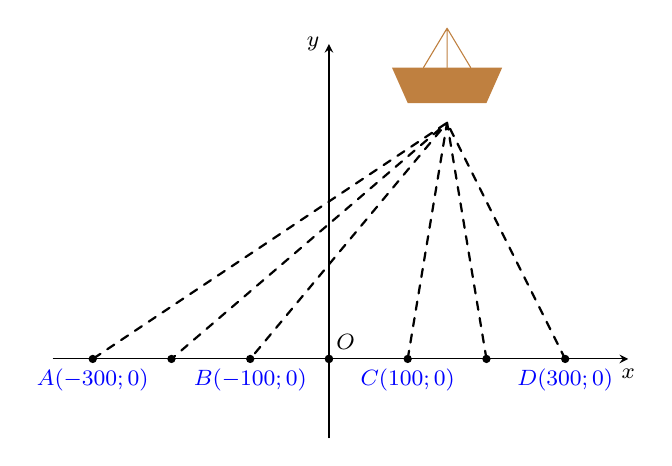
\begin{tikzpicture}[scale=1, font=\footnotesize, line join=round, line 
        cap=round, >=stealth]
        \path 
        (0,0) coordinate (O);
        
        %   \draw[gray!50] (-3,-3) grid (5,5);
        \draw[->] (-3.5,0)--(3.8,0) node[below]{$x$};
        \draw[->] (0,-1)--(0,4) node[left]{$y$};
        \draw[thick,dashed] (3,0)--(1.5,3)--(-3,0) (2,0)--(1.5,3)--(-2,0) 
        (1,0)--(1.5,3)--(-1,0);
        \draw[color=blue] (-3,0) node[below]{$A(-300;0)$}  (-1,0) 
        node[below]{$B(-100;0)$} 
        (3,0)   node[below]{$D(300;0)$} (1,0) node[below]{$C(100;0)$};
        \fill[color=brown] (0.8,3.7)--(1,3.25)--(2,3.25)--(2.2,3.7)--cycle ;
        \draw[color=brown](1.2,3.7)--(1.5,4.2)--(1.8,3.7) (1.5,4.2)--(1.5,3.7);
        \foreach \p/\r in {O/45}
        \fill (\p) circle (1.5pt) node[shift={(\r:3mm)}]{$\p$};
        \foreach \q in {-3,-2,-1,0,1,2,3}   \fill (\q,0) circle (1.5pt) ;
    \end{tikzpicture}
 \end{center}
    \begin{enumerate}
        \item Tính hiệu các khoảng cách từ tàu đến các trạm $B$, $C$.
        \item Tính hiệu các khoảng cách từ tàu đến các trạm $A$, $D$.
        \item Chọn hệ trục tọa độ $Oxy$ như hìn vẽ ($1$ đơn vị trên mặt phẳng toạ độ ứng với $100$ km trên thực tế). Hãy lập phương trình chính tắc của hai hypebol đi qua vị trí $M$ của tàu. Từ đó, tính toạ độ của $M$ (các số được làm tròn đến hàng đơn vị).
        \item Tính các khoảng cách từ tàu đến các trạm $B, C$ (đáp số được làm tròn đến hàng đơn vị, tính theo đơn vị km).
    \end{enumerate}

    \loigiai{
            \begin{itemize}
            \item Gọi vận tốc phát tín hiệu là $v$ (theo đề bài $v =292000$ km/s).
            \item $t_A, t_B, t_C, t_D$ lần lượt là thời gian để tàu nhận được tín hiệu từ các trạm $A, B, C, D$.
            \item $M$ là vị trí của tàu thủy.
        \end{itemize}
\begin{enumerate}
    \item Hiệu các khoảng cách từ tàu đến các trạm $B, C$ là 
    $$MB-MC=v \cdot t_B-v \cdot t_C=v\left(t_B-t_C\right)=292000 \cdot 0{,}0005=146\, \mathrm{km }.$$
    \item Hiệu các khoảng cách từ tàu đến các trạm $A, D$ là
    $$  M A-M D=v \cdot t_D-v \cdot t_A=v\left(t_D-t_A\right)=292000 \cdot 0,001=292 \,\mathrm{km }.
    $$  
    \item 
    \begin{itemize}
        \item Gọi phương trình chính tắc của hypebol $(\left.\mathrm{H}_1\right)$ nhận $B, C$ làm tiêu điểm là $$\dfrac{x^2}{a_1^2}-\dfrac{y^2}{b_1^2}=1\left (a_1>0, b_1>0\right).$$
        Vi $MB - MC = 146$ nên $2 a_1=146 \Rightarrow a_1=73 \Rightarrow a_1^2=5329$.\\
        Ta thấy $B(-100 ; 0)$ và $C(100 ; 0)$ là hai tiêu điểm của hypebol nên\\ $c_1=100$ $\Rightarrow b_1^2=c_1^2-a_1^2=100^2-73^2=4671$.\\
        Vậy phương trình chính tắc của hypebol $\left(\mathrm{H}_1\right)$ là $\dfrac{x^2}{5329}-\dfrac{y^2}{4671}=1$.
        \item Gọi phương trình chính tắc của hypebol  $(\left.\mathrm{H}_2\right)$ nhận $A, D$ làm tiêu điểm
        là $$\dfrac{x^2}{a_2^2}-\dfrac{y^2}{b_2^2}=1 \,\left(a_2>0, ~b_2>0\right).$$
        Vì $MA - MD =29{,}2$ nên $2 a_2=292 \Rightarrow a_2=146 \Rightarrow a_2^2=21316$.\\
        Ta thấy $A(-300 ; 0)$ và $D(300 ; 0)$ là hai tiêu điểm của hypebol nên \\$c_2=300$ $\Rightarrow b_2^2=c_2^2-a_2^2=300^2-146^2=68684$.\\
        Vậy phương trình chính tắc của hypebol $\left(\mathrm{H}_2\right)$ là $\dfrac{x^2}{21316}-\dfrac{y^2}{68684}=1$.\\
        Gọi toạ độ của $M$ là $(x ; y)$. Vì $M$ thuộc cả $\left(\mathrm{H}_1\right)$ và $\left(\mathrm{H}_2\right)$ nên ta có:
        $$\left\{\begin{aligned} 
        & \dfrac {x^2}{5 3 2 9} - \dfrac{y^2}{ 4 6 7 1 } = 1  \\
        & \dfrac {x^2}{ 2 1 3 1 6} - \dfrac {y^2}{6 8 6 8 4}= 1
        \end{aligned}\right.
        \Rightarrow \left\{\begin{aligned}  
        &{ x ^ { 2 } = \dfrac { 3 4 1 1 2 5 2 7 7 } { 1 2 5 0 0 } } \\
        &{ y ^ { 2 } = \dfrac { 2 4 0 6 1 7 2 2 3 } { 1 2 5 0 0 } }
    \end{aligned}\right.   \Rightarrow \left\{\begin{aligned}
        &x \approx 165 \\
        &y \approx 139.
    \end{aligned}\right.$$
        (vì theo hình vẽ $x, y>0$ )
    \end{itemize} 
    \item  $M B=\sqrt{[165-(-100)]^2+(139-0)^2} \approx 299$ km. \\
    $M C=\sqrt{(165-100)^2+(139-0)^2} \approx 153\,\mathrm{~km}$.
\end{enumerate}
    
    }
\end{vd}

\begin{vd}%[0H7KL-0]%[0H7TL-0]
    Nhờ việc thu tín hiệu từ hai trạm phát sóng $A$ và $B$ trên bờ, hệ thống định vị đặt tại điểm $M$ trên con tàu tính được hiệu số khoảng cách từ $M$ đến $A, B$ và xác định được một đường hypebol đi qua $M$. Cho biết khoảng cách giữa hai trạm vô tuyến là $600$km, vận tốc sóng vô tuyến là $300000$km/s và thời gian con tàu nhận được tín hiệu từ hai trạm trên bờ biển luôn cách nhau $0{,}0012$s (hai trạm vô tuyến phát các tín hiệu cùng một thời điểm). Viết phương trình chính tắc của quỹ đạo hypebol (H) của con tàu.
    \begin{center}
        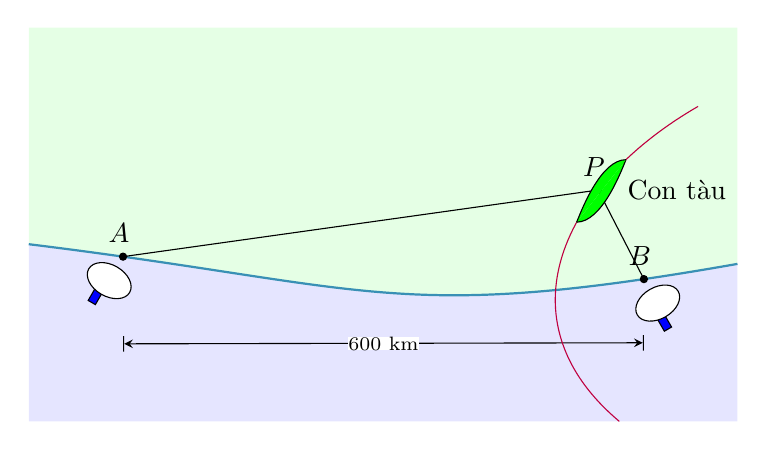
\begin{tikzpicture}[>=stealth]
            \def\bomot{(-3,5)--(6,5)}
            \def\bohai{(6,2)to [out=-170,in=-7,looseness=1.25] +(-9,0.25)}
            \def\boba{(-3,0)--(6,0)}
            \path
            (6,2)to [out=-170,in=-7,looseness=1.25] coordinate[pos=0.9](A)  +(-9,0.25) 
            (6,2)to [out=-170,in=-7,looseness=1.25] coordinate[pos=0.1](B) +(-9,0.25) ;
            \begin{scope}
                \clip (-3,0) rectangle (6,5);
                \fill[color=white!90!blue] \bohai--\boba--cycle;
                \fill[color=white!90!green] \bohai--\bomot--cycle;
            \end{scope}
            %\draw[gray!50] (-3,0) grid (6,5);
            \draw[thick,cyan!70!black] \bohai ;
            \draw[fill=blue,rotate=-30] ([yshift=-10pt]A) rectangle 
            ([xshift=-3pt,yshift=-20pt]A);
            \draw[fill=white,rotate=-30] ([yshift=-10pt]A) ellipse ({0.3} and {0.2});
            \draw[fill=blue,rotate=30] ([yshift=-10pt]B) rectangle 
            ([xshift=-3pt,yshift=-20pt]B);
            \draw[fill=white,rotate=30] ([yshift=-10pt]B) ellipse ({0.3} and {0.2});
            \begin{scope} 
                \draw[|<->|] ([yshift=-31.5pt]A) -- ([yshift=-23pt]B)
                node[midway,fill=white,inner sep=0pt]{\scriptsize$ 600 $ km} ;
            \end{scope}
            \draw[purple] (4.5,0)..controls +(140:2) and +(210:2)..(5.5,4) 
            coordinate[pos=0.7](P) coordinate[pos=0.6](N) coordinate[pos=0.8](H);
            \draw (A)--(P)--(B);
            \draw ([xshift=1cm]P) node{Con tàu};
            \foreach \p/\r in {A/100,B/100,P/100}
            \fill (\p) circle (1.5pt) node[shift={(\r:3mm)}]{$\p$};
            \draw[fill=green] (H) parabola [bend at end] (N);
            \draw[fill=green] (N) parabola [bend at end] (H);
        \end{tikzpicture}
    \end{center}
    \loigiai{
    \begin{itemize}
        \item Chọn hệ trục toạ độ sao cho gốc toạ độ $O$ trùng với tiêu điểm của $AB$, đơn vị trên các trục là km.  
        \item Giả sử phương trình chính tắc của $(\mathrm{H})$ là $\dfrac{x^2}{a^2}-\dfrac{y^2}{b^2}=1\, (a>0,b>0)$.
        \item   Gọi $t_1$ là thời gian con tàu nhận được tín hiệu từ trạm $A$; $t_2$ là thời gian con tàu nhận được tín hiệu từ trạm $B$, $v$ là vận tốc sóng vô tuyến.     Theo đề bài ta có: $\left|t_1-t_2\right|=0{,}0012$.
        $$
        \begin{aligned}
            &\Rightarrow\left|vt_1-vt_2\right|=0{,}0012 v=0{,}0012\cdot 300000=360 \,(\mathrm{km}) \\
            &\Rightarrow\left|MA-MB\right|=360 \text { với mọi vị trí của } M \\
            &\Rightarrow 2 a=360 \Rightarrow a=180.
        \end{aligned}
        $$
        \item Có khoảng cách giữa hai trạm vô tuyến là $600 \mathrm{~km} \Rightarrow 2c=600 \Rightarrow c=300$ $\Rightarrow b^2=c^2-a^2=300^2-180^2=57600$.
        \item   Vậy phương trình chính tắc của $\mathrm{(H)}$ là $\dfrac{x^2}{32400}-\dfrac{y^2}{57600}=1$.
        \end{itemize}
    }
\end{vd}
\begin{vd}%[0H7GL-0]%[0H7TL-0]
    Một vật thể có quỹ đạo là một nhánh của hypebol (H), nhận tâm Mặt Trời làm tiêu điểm. Cho biết tâm sai của $(\mathrm{H})$ bằng $1{,}2$ và khoảng cách gần nhất giữa vật thể và tâm Mặt Trời là $2\cdot 10^8 \mathrm{~km}$.
    \begin{enumerate}
    \item Lập phương trình chính tắc của $(\mathrm{H})$.
    \item Lập công thức tính bán kính qua tiêu của vị trí $M(x;y)$ của vật thể trong mặt phẳng toạ độ.
    \end{enumerate}
    \loigiai{
        \begin{center}
        \begin{tikzpicture}[scale=1, font=\footnotesize, line join=round, line 
            cap=round, >=stealth]
            \path 
            (0.4,2) coordinate (F)
            ;
            %\draw[gray!50] (-3,-3) grid (5,5);
            \draw[green] (0.5,0)..controls +(120:2) and +(210:2)..(1,4) 
            coordinate[pos=0.9](M);
            \draw (M)--(F);
            \fill[yellow] (0.4,2) circle (0.3cm);
            \fill[red] (0.4,2) circle (0.15cm);
            \draw (1.4,2) node{Mặt trời}  (-0.3,2.7) ;
            \foreach \p/\r in {M/180}
            \fill (\p) circle (1.5pt) node[shift={(\r:3mm)}]{$\p$};
            \fill (F) node[shift={(-110:5mm)}]{$F$};
        \end{tikzpicture}
        \end{center}
    \begin{enumerate}
        \item  
        \begin{itemize}
            \item Chọn hệ trục toạ độ sao cho tiêu điểm $F_2$ của (H) trùng với tâm Mặt Trời, trục $Ox$ đi qua đỉnh và tiêu điểm này của (H), đơn vị trên các trục là $\mathrm{km}$.
            \item Gọi phương trình chính tắc của (H) là $\dfrac{x^2}{a^2}-\dfrac{y^2}{b^2}=1 \,(a>0, b>0)$. Gọi toạ độ của vật thể là $M(x ; y)$.
            \item   Áp dụng công thức bán kính qua tiêu, ta có khoảng cách giữa vật thể và tâm Mặt Trời là $MF_2=\left|a-\dfrac{c}{a} x\right|=|a-e x|=ex-a \geq ea - a$ (vì vật thể nằm ở nhánh bên phải trục $Ox$ nên $x \geq a$).
            \item Như vậy khoảng cách gần nhất giữa vật thể và tâm Mặt Trời là $ea - a$ $\Rightarrow$ $ea -a=2 \cdot 10^8 \Rightarrow 1{,}2 a-a=2 \cdot 10^8 \Rightarrow a=10^9 \Rightarrow c= ea =1{,}2 \cdot 10^9$ $\Rightarrow b^2=c^2-a^2=\left(1{,}2\cdot 10^9\right)^2-\left(10^9\right)^2=0{,}44\cdot 10^{18}$.
            \item Vậy phương trình chính tắc của $(\mathrm{H})$ là $\dfrac{x^2}{10^{18}}-\dfrac{y^2}{0{,}44\cdot10^{18}}=1$.
        \end{itemize} 
    \item Bán kính qua tiêu của vị trí $M(x;y)$ của vật thể trong mặt phẳng toạ độ là
    $$
    MF_2=\left|a-\dfrac{c}{a} x\right|=|a-e x|=\left|10^9-1{,}2 x\right| \,(\mathrm{km}).
    $$
\end{enumerate} 
    }
\end{vd}

\begin{vd}%[0H7GL-0]%[0H7TL-0]
Dọc theo bờ biển, người ta thiết lập hệ thống định vị vô tuyến dẫn đường tâm xa để truyền tín hiệu cho máy bay hoặc tàu thuỷ hoạt động trên biển. Trong hệ thống đó có hai đài vô tuyến đặt lần lượt tại địa điểm $A$ và địa điểm $B$, khoảng cách $A B=650$ km. Giả sử có một con tàu chuyển động trên biển với quỹ đạo là hypebol nhận $A$ và $B$ là hai tiêu điểm. Khi đang ở vị trí $P$, máy thu tín hiệu trên con tàu chuyển đổi chênh lệch thời gian nhận các tín hiệu từ $A$ và $B$ thành hiệu khoảng cách $\mid P A$ - $P B \mid$. Giả sử thời gian con tàu nhận được tín hiệu từ $B$ trước khi nhận được tín hiệu từ $A$ là $0{,}0012$ s. Vận tốc di chuyển của tín hiệu là $3\cdot 10^8$ m/s.
    \begin{center}
    \begin{tikzpicture}[>=stealth]
        \def\bomot{(-3,5)--(6,5)}
        \def\bohai{(6,2)to [out=-170,in=-7,looseness=1.25] +(-9,0.25)}
        \def\boba{(-3,0)--(6,0)}
        \path
        (6,2)to [out=-170,in=-7,looseness=1.25] coordinate[pos=0.9](A)  +(-9,0.25) 
        (6,2)to [out=-170,in=-7,looseness=1.25] coordinate[pos=0.1](B) +(-9,0.25) ;
        \begin{scope}
            \clip (-3,0) rectangle (6,5);
            \fill[color=white!90!blue] \bohai--\boba--cycle;
            \fill[color=white!90!green] \bohai--\bomot--cycle;
        \end{scope}
        %\draw[gray!50] (-3,0) grid (6,5);
        \draw[thick,cyan!70!black] \bohai ;
        \draw[fill=blue,rotate=-30] ([yshift=-10pt]A) rectangle 
        ([xshift=-3pt,yshift=-20pt]A);
        \draw[fill=white,rotate=-30] ([yshift=-10pt]A) ellipse ({0.3} and {0.2});
        \draw[fill=blue,rotate=30] ([yshift=-10pt]B) rectangle 
        ([xshift=-3pt,yshift=-20pt]B);
        \draw[fill=white,rotate=30] ([yshift=-10pt]B) ellipse ({0.3} and {0.2});
        \begin{scope} 
            \draw[|<->|] ([yshift=-31.5pt]A) -- ([yshift=-23pt]B)
            node[midway,fill=white,inner sep=0pt]{\scriptsize$ 650 $ km} ;
        \end{scope}
        \draw[purple] (4.5,0)..controls +(140:2) and +(210:2)..(5.5,4) 
        coordinate[pos=0.7](P) coordinate[pos=0.6](N) coordinate[pos=0.8](H);
        \draw (A)--(P)--(B);
        \draw ([xshift=1cm]P) node{Tàu thủy};
        \foreach \p/\r in {A/100,B/100,P/100}
        \fill (\p) circle (1.5pt) node[shift={(\r:3mm)}]{$\p$};
        \draw[fill=green] (H) parabola [bend at end] (N);
        \draw[fill=green] (N) parabola [bend at end] (H);
    \end{tikzpicture}
\end{center}
\begin{enumerate}
    \item Lập phương trình hypebol mô tả quỹ đạo chuyển động của con tàu.
    \item Chứng tỏ rằng tại mọi thời điểm trên quỹ đạo chuyển động thì thời gian con tàu nhận được tín hiệu từ $B$ trước khi nhận được tín hiệu từ $A$ luôn là $0{,}0012$ s.
\end{enumerate}
    \loigiai{
    
    \begin{enumerate}
    \item 
    \begin{itemize}
        \item   Vì thời gian con tàu nhận được tín hiệu từ  $B$ trước khi nhận được tín hiệu từ $A$ là $0{,}0012 \mathrm{~s}$ nên tại thời điểm đó $PB-PA=\left(3 \cdot 10^8\right) \cdot 0{,}0012=$ $360000 \, (\mathrm{m})=360 \,(\mathrm{km})$.
        \item   Vì con tàu chuyển động với quỹ đạo là hypebol nhận $A$ và $B$ là hai tiêu điểm nên $\mid P A - PB \mid=360 \,(\mathrm{km})$ với mọi vị trí của $P$.
        \item  Chọn hệ trục toạ độ sao cho gốc toạ độ trùng với trung điểm của $A B$ và trục $Ox$ trùng với $A B$, đơn vị trên hai trục là km thì hypebol này có dạng $\dfrac{x^2}{a^2}-\dfrac{y^2}{b^2}=1 \,(a>0,  b>0)$.
        \item Vì $|PA-PB|=360$ nên $2a=360$, suy ra $a=180$.\\
        Theo đề bài, $AB=650$, suy ra $2c=650$, suy ra $c=325$.
        $$
        b^2=c^2-a^2=325^2-180^2=73225.  $$
        \item   Vậy phương trình hypebol mô tả quỹ đạo chuyển động của con tàu là $\dfrac{x^2}{32400}-\dfrac{y^2}{73225}=1.$    
    \end{itemize}

    \item 
    \begin{itemize}
        \item Vì con tàu chỉ chuyển động ở nhánh bên phải trục $Oy$ của hypebol nên ta $PB < PA$ với mọi vị trí của $P$. Do đó tàu luôn nhận được tín hiệu từ $B$ trước khi nhận được tín hiệu từ $A$.
        \item Gọi $t_1$ là thời gian để tàu nhận được tín hiệu từ $A$, $t_2$ là thời gian để tàu nhận được tín hiệu từ $B$ thì $t_1=\dfrac{PA}{v}, t_2=\dfrac{PB}{v}$ với $v$ là vận tốc di chuyển của tín hiệu. Khi đó, ta có:
        $$
        t_1-t_2=\dfrac{PA-PB}{v}=\dfrac{360000}{3 \cdot 8^{10}}=0{,}0012\,(\mathrm{s}).
        $$
        \item   Vậy thời gian con tàu nhận được tín hiệu từ $B$ trước khi nhận được tín hiệu từ $A$ luôn là $0{,}0012$ s.
    
    \end{itemize}
    
    \end{enumerate} 
    

    }
\end{vd}











    
